\section{Macierz Seiferta} % (fold)
W tej sekcji pogłębimy nasze rozumienie wielomianu Alexandera i~odkryjemy jego powiązania z topologicznymi własnościami węzłów.
Poznamy także zupełnie nowy sposób na wyznaczanie jego wartości,
Jak nie jest trudno się domyślić, posłuży do tego macierz Seiferta.

\subsection{Powierzchnia Seiferta}
Zaczniemy od przyjrzenia się powierzchniom.
Niektóre stwierdzenia będziemy przyjmować bez dowodu, by nie rozwodzić się za bardzo nad topologią algebraiczną.

\begin{definition}
    \index{powierzchnia}
    Powierzchnia to dwuwymiarowa rozmaitość topologiczna $M \subseteq \R^3$.
\end{definition}

Rozmaitość to obiekt, który wygląda lokalnie jak przestrzeń euklidesowa: każdy jej punkt $x \in M$ posiada otwarte otoczenie homeomorficzne z~otwartą kulą.
Przykładami powierzchni są sfera, brzeg torusa albo hiperboloida jednopowłokowa.
Istnieje ogólniejsze pojęcie, to jest rozmaitość z~brzegiem: każdy jej punkt posiada otoczenie homeomorficzne z otwartym podzbiorem górnej półpłaszczyzny $\{x \in \C: \mathfrak {Im} \ge 0\}$.
Zwartą powierzchnię bez brzegu nazywamy \emph{domkniętą}.

Powierzchnię nazywamy orientowalną, jeśli nie istnieje na niej zamknięta krzywa, podczas pokonywania której odwraca się kierownica.
Orientowalne są dokładnie te powierzchnie, które nie zawierają w sobie kopii wstęgi Möbiusa.

Najważniejsze dla nas są powierzchnie Seiferta:

\begin{definition}
\index{powierzchnia!Seiferta}
    Powierzchnia Seiferta związana z~węzłem $K$ to spójna,
    orientowanlna powierzchnia zanurzona w~$\R^3$, której brzegiem jest $K$.
\end{definition}

% \begin{example}
% Powierzchnia Seiferta dla trójlistnika:
% \begin{center}
% \begin{tikzpicture}
% [scale=0.1]
%   \clip (-17,-15) rectangle (17,15);
%   \foreach \d in {0,180} {
%       \path[OBSZAR    ,rotate=\d] (-1.25,11.5)
%       .. controls (2,14) and (6,13.5) ..  (10,12)
%       .. controls (23,7) and (15,-20)  .. (3,-13)
%       -- (1.25, -11.5)
%       .. controls (4.5,-8) and (4.5,-4) .. (0,0)
%       .. controls (4,4) and (4.5,5.5) .. (-1.25,11.5);}
%   \path[TIKZ_ARCH] (0,10) .. controls (10,0) and (-10,0) .. (0,-10);
%   \foreach \d in {0,180} {
%   \path[TIKZ_ARCH, rotate=\d] (-1.5,1.5) .. controls (-6,6) and (-3,17) .. (10,12)
%   .. controls (23,7) and (15,-20)  .. (3,-13);}
% \end{tikzpicture}
% \end{center}
% \end{example}

Nie każde uszachowienie diagramu węzła prowadzi do powierzchni Seiferta:
widać to po standardowym diagramie trójlistnika.
Pomimo to...

\begin{proposition}
    \label{seifert_existence}
    Każdy węzeł posiada powierzchnię Seiferta.
\end{proposition}

Powyższe stwiedzenie uzasadnili Pontriagin oraz Frankl w~1930 roku, my jednak podamy bardzo przyjemny i~konstruktywny dowód podany przez Seiferta cztery lata później.

\begin{proof}
    Wybierzmy diagram $D$ dla węzła oraz orientację,
    a~następnie wyprostujmy wszystkie skrzyżowania zgodnie z~ich orientacją:

    \[
    \begin{tikzpicture}[scale=0.12, baseline=-3]
        \begin{knot}[clip width=15, end tolerance=1pt,flip crossing/.list={1}]
            \strand[semithick,Latex-] (-5,5) to (5,-5);
            \strand[semithick,-Latex] (-5,-5) to (5,5);
        \end{knot}
    \end{tikzpicture}
    \quad\longrightarrow\quad
        \begin{tikzpicture}[baseline=-0.65ex, scale=0.12]
        \useasboundingbox (-5, -6) rectangle (5, 6);
        \draw[semithick,-Latex] (-4, -5) to [out=45, in=-45] (-4, 5);
        \draw[semithick,-Latex] (4, -5) to [out=135, in=-135] (4, 5);
        \end{tikzpicture}
        \quad\longleftarrow\quad
    \begin{tikzpicture}[scale=0.12, baseline=-3]
        \begin{knot}[clip width=15, end tolerance=1pt]
            \strand[semithick,Latex-] (-5,5) to (5,-5);
            \strand[semithick,-Latex] (-5,-5) to (5,5);
        \end{knot}
    \end{tikzpicture}
    \]

    Otrzymany diagram składa się teraz z~pewnej liczby zamkniętych krzywych,
    zwanych okręgami Seiferta, które wypełniamy do dysków.
    Tam, gdzie jeden okrąg leżał wewnątrz drugiego, podnosimy wewnętrzny nad zewnętrzny.
    Przy każdym skrzyżowaniu pierwotnego diagramu doklejamy skręcony pasek do obydwu dysków.

    Dyski są dwustronne, więc ich górnej stronie przypisujemy znak $+$,
    jeśli tylko brzeg jest zorientowany dodatnio i~$-$ w~przeciwnym razie.

    \begin{center}
        %\includegraphics[width=0.75\textwidth]{seifert.png}
        (brakująca grafika)
    \end{center}
\end{proof}

Powierzchnia Seiferta dziedziczy orientację po węźle.
Nawet niewinne odwrócenie jednego z ogniw splotu potrafi istotnie zmienić jego powierzchnię, dlatego potrzebna jest ostrożność!
Zanim przejdziemy do zdefiniowania macierzy Seiferta, potrzebować będziemy krótkiego skoku w bok -- zrozumieć bardzo geometryczny niezmiennik węzłów, genus.

\subsection{Genus} % (fold)
\label{sec:genus}
Zaczniemy od starego twierdzenia, które klasyfikuje powierzchnie domknięte.

\begin{proposition}
    Każda powierzchnia domknięta jest członkiem jednej z dwóch nieskończonych rodzin:
    \begin{enumerate}[leftmargin=*]
        \itemsep0em
        \item sumą spójną $g \ge 0$ torusów,
        \item sumą spójną $k \ge 1$ rzeczywistych płaszczyzn rzutowych.
    \end{enumerate}
\end{proposition}

Elementy pierwszej rodziny są orientowalne.
Sferę traktujemy dla wygody jako sumę spójną $g = 0$ torusów.
Wtedy sumę spójną $g$ torusów możemy wyobrazić sobie jako sferę, do której doklejono $g$ uchwytów.

\begin{definition}[genus powierzchni]
    Ilość torusów nazywamy genusem powierzchni i oznaczamy literą $g$.
\end{definition}

Podobna charakteryzacja istnieje dla powierzchni z~brzegiem.
Każdy taki obiekt jest homeomorficzny z~sumą spójną $g$ torusów, w~których wydrążono pewną liczbę otworów: tyle, ile składowych spójności ma brzeg powierzchni.
W~przypadku powierzchni Seiferta mamy do czynienia z jednym otworem.

Dla wygody przypomnijmy jeszcze definicję klasycznego niezmiennika powierzchni:

\begin{definition}[charakterystyka Eulera]
    \index{charakterystyka Eulera}
    Niech $M$ będzie domkniętą powierzchnią orientowalną.
    Po striangulowaniu, składa się z $k_0$ wierzchołków, $k_1$ krawędzi oraz $k_2$ ścian.
    Wielkość
    \begin{equation}
        \chi = k_0 - k_1 + k_2
    \end{equation}
    jest niezmiennikiem powierzchni, zwanym zazwyczaj charakterystyką Eulera.
\end{definition}

Jeśli $M$ jest powierzchnią o genusie $g$ i $\mu$ składowych spójności brzegu, to $\chi = 2 - \mu - 2g$.
Nas interesują głównie powierzchnie Seiferta węzłów:

\begin{proposition}
    Niech $K$ będzie węzłem z~diagramem $D$.
    Wtedy $\chi(M_D) = d - b$, gdzie $b$ jest liczbą skrzyżowań $D$, zaś $d$ jest liczbą okręgów Seiferta.
\end{proposition}

\begin{proof}
    W~dowodzie faktu \ref{seifert_existence} widzieliśmy, że liczba skrzyżowań $b$ jest jednocześnie liczbą pasków doklejonych do dysków.
    Bezpośredni rachunek pokazuje, że wtedy $k_0 = 4b$, $k_1 = 6b$ oraz $k_2 = b+d$.
    Wynika stąd, że $\chi = 4b - 6b + b + d = d - b$.
\end{proof}

Reszta tej podsekcji nie jest wymagana do zrozumienia macierzy Seiferta, przyjrzymy się genusowi jako obiektowi ciekawemu samemu w sobie.

\begin{definition}[3-genus]
    Niech $K$ będzie węzłem.
    Minimalny genus spośród wszystkich powierzchni Seiferta węzła $K$ nazywamy 3-genusem i oznaczamy $g$.
\end{definition}

Znalezienie 3-genusu dowolnego węzła sprawia te same trudności, co wyznaczenie jego liczby gordyjskiej.
Dowolna powierzchnia Seiferta zadaje ograniczenie z góry.
Z dołu 3-genus można szacować przy użyciu wielomianu Alexandera:

\begin{proposition}
    Niech $K$ będzie węzłem.
    Wtedy $\operatorname{span} \Delta(t) \le 2g$.
\end{proposition}

To dolne ograniczenie jest realizowane przez pewną powierzchnię Seiferta dla każdego pierwszego węzła o~co najwyżej 11 skrzyżowaniach poza siedmioma wyjątkami: 11n42, 11n67, 11n97 ($g = 2$), 11n34, 11n45, 11n73 oraz 11n152 ($g=3$).
Jeżeli nie powoduje to nieporozumień, zamiast 3-genus można pisać po prostu genus.

Czy w definicji genusu można ograniczyć się do powierzchni Seiferta, które pochodzą od algorytmu Seiferta?
Niestety, poza pewnymi wyjątkami, nie.
Zanim przekonamy się, dlaczego tak jest, zdefiniujmy jeszcze dwa niezmienniki.

\begin{definition}[genus kanoniczny]
    Niech $K$ będzie węzłem.
    Minimalny genus spośród wszystkich powierzchni Seiferta węzła $K$, które pochodzą z~algorytmu Seiferta, nazywamy genusem klasycznym i~oznaczamy $g_c$.
\end{definition}

Pod koniec lat pięćdziesiątych Crowell i~Murasugi niezależnie zauważyli, że algorytm Seiferta zastosowany do alternującego diagramu zawsze daje powierzchnię o~minimalnej powierzchni.
Ich kombinatoryczne uzasadnienie było dość zawiłe, elementarny dowód podał Gabai w \cite{gabai86}.

Dubel trójlistnika ma genus równy $1$, ale algorytm Seiferta zastosowany wobec węzła produkuje powierzchnie o genusie co najmniej $3$, jak przewiduje ograniczenie znalezione przez Mortona w \cite{morton86} jako twierdzenie 2:

\begin{proposition}
    Niech $P(v, z)$ będzie wersją wielomianu HOMFLY spełniającą zależność
    \begin{equation}
        \frac 1v P_+ - vP_- = zP_0.
    \end{equation}
    Wtedy $M = \max \deg_z P(v, z) \le 2g_c$.
\end{proposition}

Nierówność Mortona jest równością dla wielu klas węzłów, w tym alternujących (Crowell, Murasugi), jednorodnych (które stanowią uogólnienie węzłów alternujących, Crowell w \cite{cromwell89}), whiteheadowskich dubli węzłów dwumostowych (Nakamura w \cite{nakamura06}, Tripp w \cite{tripp02}) albo precli (Brittenham w \cite{brittenham07}).
Stojmenow pokazał, że staje się równością dla węzłów o co najwyżej 12 skrzyżowaniach i znalazł przykład węzła, dla którego jest ostra.

\begin{definition}[genus wolny]
    Niech $K$ będzie węzłem.
    Minimalny genus spośród powierzchni Seiferta węzła $K$, których dopełnienie w 3-sferze jest \emph{ciałem z rączkami} (handlebody, czyli ma wolną grupę podstawową), nazywamy genusem wolnym i~oznaczamy $g_f$.
\end{definition}

Dopełnienie powierzchni Seiferta jest zawsze handlebody, dlatego też mamy oczywiste nierówności $g \le g_f \le g_c$.
Morton w 1986 roku pokazał, że genus pewnych węzłów nie jest realizowany przez żaden diagram do którego stosuje się algorytm Seiferta, choćby $10_{165}$.
Patrz \cite{morton86}.
Moriah, matematyk izraelski, mniej więcej w tym samym czasie rozwiązał problem postawiony dekadę wcześniej przez Kirby'ego \cite{kirby78}: jak duża może być różnica $g_f - g$?

\begin{proposition}
    Niech $K$ będzie węzłem, $D_k(K)$ jego dublem Whiteheada z $k \neq 0$ skręceniami, zaś $B_n(K)$ to $n$-krotne nakrycie cykliczne sfery $S^3$ rozgałęzione nad węzłem $K$.
    Jeżeli ranga pierwszej grupy homologii $B_{|4k+1|}(K)$ wynosi $r$, to
    \begin{equation}
        g_f(D_k(K)) \ge \frac {2r-1} {|8k+2|}.
    \end{equation}
\end{proposition}

\begin{proof}
    Praca \cite{moriah87}.
    Dowód opiera się na chirurgii węzłów i splotów w sferze $S^3$.
\end{proof}

\begin{corollary}
    Niech $K$ bedzie sumą spójną $n$ trójlistników, połóżmy $k = -1$.
    Wtedy pierwsza grupa homologii ma rangę $r = 2n$ i~genus wolny jest nieograniczony
    \begin{equation}
        g_f(D_{-1}(3_1^n)) \ge \frac {4n-1} {6},
    \end{equation}
    podczas gdy zwykły genus to $g(D_{-1}(3_1^n)) = 1$.
\end{corollary}

\begin{proposition}
    \label{genus_one}
    Genus wykrywa niewęzły: $K$ jest niewęzłem wtedy i tylko wtedy, gdy $g(K) = 0$.
\end{proposition}

\begin{proof}
    Oto szkic dowodu.
    Jeżeli genus wynosi zero, to $K$ ma powierzchnię Seiferta o~jednej składowej brzegowej i~genusie zero.
Dysk też ma te własności, więc korzystamy z~klasyfikacji powierzchni (dysk jest powierzchnią).
\end{proof}

\begin{proposition}
\label{genus_sum}
    Jeśli $J, K$ są węzłami, to $g (J \shrap K) = g(J) + g(K)$.
\end{proposition}

\begin{proof}
    Pokażemy najpierw, że $g(J \# K) \le g(J) + g(K)$.
    Wybierzmy powierzchnie Seiferta $M_J$ oraz $M_K$ dla $J$ oraz $K$ o~minimalnym genusie.
    Suma $J \shrap K$ powstaje z~$J$ oraz $K$, podobnie jest z~powierzchniami Seiferta:
    \[
        \begin{tikzpicture}[baseline=-0.65ex,scale=0.12]
        \draw[semithick,-Latex] (-7, -5) to (-5, -5) [in=right, out=right] to (-5, 5) to (-7, 5);
        \draw[semithick,Latex-] ( 7, -5) to ( 5, -5) [in=left, out=left] to ( 5, 5) to ( 7, 5);
        \node at (-5, 0) {$J$};
        \node at (5, 0) {$K$};
        \end{tikzpicture}
        \longrightarrow
        \begin{tikzpicture}[baseline=-0.65ex,scale=0.12]
        \draw[semithick,-Latex] (-7, -5) to (-5, -5) to [out=right, in=left] (-2, -2) -- (2, -2) to [out=right, in=left] (5, -5) to (7, -5);
        \draw[semithick,Latex-] (-7, 5) to (-5,  5) to [out=right, in=left] (-2,  2) -- (2,  2) to [out=right, in=left] (5,  5) to (7, 5);
        \node at (0, -5) {$J \# K$};
        \end{tikzpicture}
        \quad\quad
        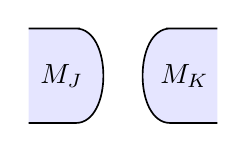
\begin{tikzpicture}[baseline=-0.65ex,scale=0.12]
        \draw[semithick,fill=blue!10!white] (-10, -5) to (-5, -5) [in=right, out=right] to (-5, 5) to (-10, 5);
        \draw[semithick,fill=blue!10!white] ( 10, -5) to ( 5, -5) [in=left, out=left] to ( 5, 5) to (10, 5);
        \node at (-6.5, 0) {$M_J$};
        \node at (6.5, 0) {$M_K$};
        \end{tikzpicture}
        \longrightarrow
        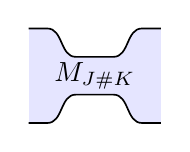
\begin{tikzpicture}[baseline=-0.65ex,scale=0.12]
        \fill[blue!10!white] (-7, -5) rectangle (7, 5);
        \draw[semithick,fill=white] (-7, -5) to (-5, -5) to [out=right, in=left] (-2, -2) -- (2, -2) to [out=right, in=left] (5, -5) to (7, -5);
        \draw[semithick,fill=white] (-7, 5) to (-5,  5) to [out=right, in=left] (-2,  2) -- (2,  2) to [out=right, in=left] (5,  5) to (7, 5);
        \node at (0, 0) {$M_{J \# K}$};
        \end{tikzpicture}
    \]

    Skoro $M_{J\#K}$ powstaje z~$M_J \sqcup M_K$ przez dołączenie paska do brzegu, mamy
    \[
        \chi(M_{J\#K}) = \chi(M_J \sqcup M_K) - 1 = \chi(M_J) + \chi(M_K)-1,
    \]
    a~przez to
    \[
        g(M_{J\#K}) = \frac{1-\chi(M_{J\#K})}{2} =
        \frac{1-\chi(M_{J})}{2} + \frac{1-\chi(M_{K})}{2}
        % = %g(M_J)+g(M_K)
        = g(J) + g(K).
    \]
    To kończy dowód pierwszej nierówności.
    Pokażemy jeszcze, że $g(J \# K) \ge g(J)+g(K)$.
    Zaczynamy od powierzchni Seiferta $M_{J\#K}$ dla $J\#K$ o~minimalnym genusie $g(M_{J\#K})$ równym $g(J\#K)$.
    Poprzez wykonanie chirurgii na powierzchni, możemy przyjąć specjalną postać jak w~poprzednim dowodzie:
    \[
        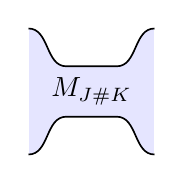
\begin{tikzpicture}[baseline=-0.65ex,scale=0.16]
            \fill[blue!10!white] (-5, -5) rectangle(5, 5);
        \draw[semithick,fill=white] (-5, -5) to [out=right, in=left] (-2, -2) -- (2, -2) to [out=right, in=left] (5, -5);
        \draw[semithick,fill=white] (-5,  5) to [out=right, in=left] (-2,  2) -- (2,  2) to [out=right, in=left] (5,  5);
            \node at (0, 0) {$M_{J \# K}$};
        \end{tikzpicture}
    \]

    Usunięcie paska daje powierzchnie Seiferta dla $M_J$ oraz $M_K$ takie, że
    \[
        g(M_J)+g(M_K)=g(M_{J\#K})=g(J\#K).
    \]
    Oznacza to, że $g(J)+g(K)\leqslant g(M_J)+g(M_K)=g(J\#K)$ i~tak naprawdę mamy równość.
\end{proof}

\begin{corollary}
\label{no_inverses}
    Jeśli suma spójna dwóch węzłów jest niewęzłem, to oba składniki także nim są.
\end{corollary}

Powrócimy teraz do węzłów pierwszych (definicja \ref{primeknot}).

\begin{proposition}
    Niech $K$ będzie węzłem.
    Jeśli $g(K) = 1$, to $K$ jest węzłem pierwszym.
\end{proposition}

\begin{proof}
    Załóżmy nie wprost, że $K = K_1 \# K_2$ jest sumą dwóch nietrywialnych węzłów.
    Z~faktu \ref{genus_sum} wynika wtedy, że $g(K) = g(K_1) + g(K_2)$.
    Zatem jeden z węzłów $K_1, K_2$ ma genus zero i jest trywialny, wbrew naszemu założeniu.
\end{proof}

Implikacja odwrotna jest fałszywa: pięciolistnik jest pierwszy, ale jego genus wynosi $2$.

\begin{proposition}
    Każdy węzeł można zapisać jako suma spójna pewnej liczby węzłów pierwszych (niewęzeł jest sumą pustej rodziny węzłów).
\end{proposition}

\begin{proof}
    Dowodzimy przez indukcję względem genusu $g(K)$.
    Przypadek bazowy $g(K) = 0$ jest oczywisty, gdyż wtedy $K$ to niewęzeł.
    Załóżmy więc, że fakt zachodzi dla węzłów $J$ genusu co najwyżej $n$.
    Niech $K$ będzie genusu $n + 1$.

    Jeśli $K$ jest pierwszy, nie ma czego dowodzić.
    W przeciwnym razie jest równoważny z~$J_1 \shrap J_2$, gdzie $J_1$ i~$J_2$ są nietrywialne.
    Mamy $g(J_1)+g(J_2)=g(K)$ oraz $g(J_1),g(J_2)\geqslant 1$.
    Zatem $g(J_1),g(J_2)\leqslant n$.
    Na mocy hipotezy indukcyjnej, $J_1$ oraz $J_2$ są równoważne sumom
    \[
        J_1 \cong K_1\#\cdots\# K_s,\qquad
        J_2 \cong K_{s+1}\#\cdots\# K_r,
    \]
    gdzie $K_i$ są pierwsze.
    Zatem $K$ jest równoważny z~$K_1\#\cdots\# K_r$, co kończy dowód.
\end{proof}

\begin{proposition}
\label{infty_primes}
    Istnieje nieskończenie wiele węzłów pierwszych.
\end{proposition}

\begin{proof}
    Pokażemy, że wszystkie węzły $(2n+2)_1$ są pierwsze, gdzie $n \ge 1$.
    Istotnie, algorytm Seiferta zastosowany do diagramu tego węzła wyprodukuje $2n+1$ okręgów.
    \[
        \begin{tikzpicture}[baseline=-0.65ex,scale=0.055]
        \begin{knot}[clip width=10, flip crossing/.list={1,4,5},end tolerance=1pt]
            \node at (0,10) {$\cdots$};
            \strand[semithick] (-30, -5) -- (-5, -5);
            \strand[semithick,-Latex]  (5, -5) -- (30, -5);
            \strand[semithick,Latex-]  (-30,-15) -- (-5,-15);
            \strand[semithick,Latex-]  (5,-15) -- (30,-15);

            \strand[semithick,domain=-90:90] plot ({7.5*cos(\x)-5}, {5*sin(\x)-10});
            \strand[semithick,domain=90:270] plot ({7.5*cos(\x)+5}, {5*sin(\x)-10});

            % zewnętrzne obręcze -- lewa strona
            \strand[semithick] (-30, 15) to [out=left, in=up]   (-45, 0);
            \strand[semithick] (-30,-15) to [out=left, in=down] (-45, 0);
            \strand[semithick] (-30,  5) to [out=left, in=up]   (-35, 0);
            \strand[semithick] (-30, -5) to [out=left, in=down] (-35, 0);

            % zewnętrzne obręcze -- prawastrona
            \strand[semithick] (30, 15) to [out=right, in=up]   (45,0);
            \strand[semithick] (30,-15) to [out=right, in=down] (45,0);
            \strand[semithick] (30,  5) to [out=right, in=up]   (35,0);
            \strand[semithick] (30, -5) to [out=right, in=down] (35,0);

            % jak w~drugim ruchu Reidemeistera - lewe
            \strand[semithick] (-30, 15) .. controls (-24, 15) and (-24,  5) .. (-20,  5);
            \strand[semithick] (-30,  5) .. controls (-24,  5) and (-24, 15) .. (-20, 15);
            \strand[semithick] (-10, 15) .. controls (-16, 15) and (-16,  5) .. (-20,  5);
            \strand[semithick] (-10,  5) .. controls (-16,  5) and (-16, 15) .. (-20, 15);

            % jak w~drugim ruchu Reidemeistera - prawe
            \strand[semithick] (30, 15) .. controls (24, 15) and (24,  5) .. (20,  5);
            \strand[semithick] (10, 15) .. controls (16, 15) and (16,  5) .. (20,  5);
            \strand[semithick] (30,  5) .. controls (24,  5) and (24, 15) .. (20, 15);
            \strand[semithick] (10,  5) .. controls (16,  5) and (16, 15) .. (20, 15);
        \end{knot}
        \end{tikzpicture}
        \longrightarrow
        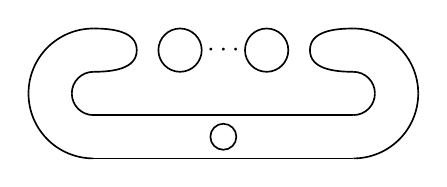
\begin{tikzpicture}[baseline=-0.65ex,scale=0.055]
            \node at (0,10) {$\cdots$};
            \draw[semithick] (-30,  -5) -- (30, -5);
            \draw[semithick] (-30, -15) -- (30,-15);

            \draw[semithick] (0,-10) circle (3);

                % zewnętrzne obręcze -- lewa strona
            \draw[semithick] (-30, 15) to [out=left, in=up]   (-45, 0);
            \draw[semithick] (-30,-15) to [out=left, in=down] (-45, 0);
            \draw[semithick] (-30,  5) to [out=left, in=up]   (-35, 0);
            \draw[semithick] (-30, -5) to [out=left, in=down] (-35, 0);

                % zewnętrzne obręcze -- prawastrona
            \draw[semithick] (30, 15) to [out=right, in=up]   (45,0);
            \draw[semithick] (30,-15) to [out=right, in=down] (45,0);
            \draw[semithick] (30,  5) to [out=right, in=up]   (35,0);
            \draw[semithick] (30, -5) to [out=right, in=down] (35,0);

            \draw[semithick] (-30, 15) to [out=right, in=up] (-20,10);
            \draw[semithick] (-30,  5) to [out=right, in=down] (-20,10);

            \draw[semithick] (30, 15) to [out=left, in=up] (20,10);
            \draw[semithick] (30,  5) to [out=left, in=down] (20,10);

            \draw[semithick] (-10, 10) circle (5);
            \draw[semithick] (10,  10) circle (5);
        \end{tikzpicture}
    \]
    Wynika stąd, że genus wynosi $\frac 12 (1 - (1+2n) + (2+2n)) = 1$, ponieważ wyznacznik ma wartość $4n+1$,
    węzły $2n+2)_1$ nie są trywialne i~są parami różne.
\end{proof}

\begin{proposition}
    Genus węzła $K$ jest związany z~wielomianem Alexandera oraz liczbą skrzyżowań:
    \[
        c(K) \ge 2 g(K) \ge \operatorname{Span}(\Delta_K(t)),
    \]
    przy czym (między innymi) dla węzłów o~co najwyżej 10 skrzyżowaniach mamy nawet równość po prawej stronie.
\end{proposition}

\index{homologia!Floera}
Wielomian Alexandera uogólnia się do (skomplikowanej) homologii Floera, pozwala ona dokładniej szacować genus węzła.

\index{węzeł!rozwłókniony}
Wspomnijmy jeszcze krótko o~specjalnym rodzaju węzłów.
Mówimy, że węzeł $K \subseteq S^3$ jest rozwłókniony\footnote{fibered}, jeśli istnieje rodzina $F_t$ powierzchni Seiferta dla $K$ sparametryzowana przez $t \in S^1$ taka, że $F_t \cap F_s = K$ dla $t \neq s$.
Dawniej nazywano je węzłami Neuwirtha.

Niewęzeł, trójlistnik i~ósemka są rozwłóknione.
Pierwszy i~ostatni współczynnik wielomianu Alexandera węzła rozwłóknionego to $\pm 1$.
Wielomianem węzła skręconego z~$q$ półskrętami jest $\Delta_q = qt - (2q+1)+q/t$, więc nie jest on rozwłókniony (dla $q \neq 1$).

% Węzeł jest rozwłókniony dokładnie wtedy, gdy stanowi grzbiet pewnego 'open book decomposition' $S^3$.

% Koniec podsekcji Genus

\subsection{Macierz Seiferta}
Niech $K$ będzie węzłem z diagramem $D$ i powierzchnią Seiferta $S$.

\begin{definition}[graf Seiferta]
    Jeżeli ściągniemy dyski z dowodu faktu \ref{seifert_existence} do punktów, zaś doklejane paski skurczymy, otrzymamy graf zwany grafem Seiferta diagramu $D$.
\end{definition}

\begin{proposition}
    Graf Seiferta jest dwudzielny i planarny.
\end{proposition}

Skoro graf Seiferta jest planarny, to dzieli sferę $S^2$ na $f$ obszarów.
Można wyznaczyć ich liczbę: skoro $\chi(S^2) = d - b + f = 2$, to $f - 1 = 1 - d + b$, pomijamy obszar nieograniczony.
Brzeg każdego obszaru jest zamkniętą krzywą, z których tworzymy krzywe $x_1, \ldots, x_m$ na powierzchni Seiferta.
Generują one grupę podstawową $\pi_1(S)$.

Niech $S$ będzie powierzchnią Seiferta z wyróżnioną jedną stroną.
Jeśli krzywa $x_i$ biegnie po powierzchni $S$, przez $x_i^*$ oznaczać będziemy dodatnie wypchnięcie: krzywą równoległą do $x_i$, która biegnie tuż nad nią.
Potrzebowaliśmy wyróżnić jedną ze stron powierzchni $S$, by słowo ,,nad'' miało sens.

\begin{definition}[macierz Seiferta]
    Przy zachowaniu powyższych oznaczeń, macierz, której wyrazy określa wzór $M_{i,j} = \operatorname{lk}(x_i, x_j^*)$, nazywamy macierzą Seiferta.
\end{definition}

Konstrukcja macierzy Seiferta zależy od wyboru diagramu oraz orientacji krzywych $x_i$, dlatego nie jest niezmiennikiem węzłów.
Stanie się nim, kiedy uwzględnimy jeszcze wpływ ruchów Reidemeistera.

\begin{definition}
    Operacja $\Lambda_1$ dla pewnej odwracalnej macierzy $P$ o całkowitych wyrazach (czyli $\det P = \pm 1$) to
    \begin{equation}
        \Lambda_1 \colon M \mapsto PMP^t.
    \end{equation}
    Natomiast
    \begin{equation}
        \Lambda_2 \colon M \mapsto \begin{bmatrix}
  &   &  & 0 & 0 \\
  & M &  & \vdots & \vdots \\
  &   &  & 0 & 0 \\
* & \dots & * & 0 & 0 \\
0 & \dots & 0 & 1 & 0
\end{bmatrix} \textrm{albo} \begin{bmatrix}
  &   &  & * & 0 \\
  & M &  & \vdots & \vdots \\
  &   &  & * & 0 \\
0 & \dots & 0 & 0 & 1 \\
0 & \dots & 0 & 0 & 0
\end{bmatrix},
    \end{equation}
    gdzie gwiazdka zastępuje ustaloną liczbę całkowitą.
\end{definition}

\begin{definition}
    Niech $M_1, M_2$ będą macierzami.
    Jeśli $M_2$ można otrzymać z $M_1$ przez skończony ciąg operacji $\Lambda_1, \Lambda_2$ oraz ich odwrotności, to macierze nazywamy $S$-równoważnymi.
\end{definition}

Litera $S$, jak nietrudno się domyślić, pochodzi od Seiferta.
Badania powyższej relacji równoważności prowadzili w~latach sześćdziesiątych ubiegłego stulecia Trotter \cite{trotter62}, Murasugi oraz Levine.

\begin{proposition}
    Macierz Seiferta modulo $S$-równoważność jest niezmiennikiem splotów.
\end{proposition}

Dowód tego faktu jest elementarny, ale dość długi.
Razem z~ułatwiającymi zrozumienie diagramami można znaleźć go w podręczniku Murasugiego, dlatego pominiemy go i skupimy się na tym, jakie niezmienniki można otrzymać z macierzy Seiferta.

Wyznacznik samej macierzy Seiferta nie jest niezmiennikiem.
Wykonując operację $\Lambda_2$ dostajemy macierz, której ostatnia kolumna albo ostatni wiersz są zerami, więc jej wyznacznik także jest zerem.
Jeśli jednak najpierw dokonamy jej symetryzacji, dostaniemy znany już niezmiennik.

\begin{proposition}
    Niech $M$ będzie macierzą Seiferta węzła $K$.
    Wtedy
    \begin{equation}
        \det K = |\det(M + M^t)|.
    \end{equation}
\end{proposition}

Przez wprowadzenie dodatkowej zmiennej $t \in \R$, ponownie uogólnimy wyznacznik do wielomianu Alexandera.

\begin{proposition}
    Niech $M$ będzie macierzą Seiferta rzędu $k$ węzła $K$.
    Wtedy
    \begin{equation}
        \Delta_K (t) = t^{-k/2}\det(M - tM^t).
    \end{equation}
\end{proposition}

Określimy jeszcze jeden, niewystępujący wcześniej niezmiennik.

\subsection{Sygnatura} % (fold)
\label{sub:signature}
\index{sygnatura}
Sygnatura pojawia się w~fakcie \ref{slice_signature}.

\begin{definition}
    Niech $M$ będzie macierzą Seiferta węzła $K$.
    Wielkość
    \begin{equation}
        \sigma K := \sigma(M + M^t)
    \end{equation}
    nazywamy sygnaturą węzła $K$.
\end{definition}

\begin{proposition} \label{prop_sigma_additive}
    Sygnatura jest addytywna: $\sigma(K_1 \shrap \ldots \shrap K_n) = \sum_{k=1}^n \sigma(K_k)$.
\end{proposition}

\begin{proof}
    Bez straty ogólności ograniczmy się do przypadku $n = 2$ i~ustalmy powierzchnie Seiferta $F_1, F_2$ dla węzłów $K_1, K_2$ z~macierzami Seiferta $M_1, M_2$.
    Powierzchnia dla ich sumy spójnej $K_1 \shrap K_2$ powstaje przez sklejenie $F_1$ oraz $F_2$ paskiem.
    W języku macierzy oznacza to, że macierz Seiferta węzła $K_1 \shrap K_2$ ma postać $M = M_1 \oplus M_2$.
    Zatem:
    \begin{equation}
        \sigma(K_1 \shrap K_2) = \sigma(M + M^t) = \sigma(M_1 + M_1^t) + \sigma(M_2 + M_2^t) = \sigma(K_1) + \sigma(K_2),
    \end{equation}
    co kończy dowód.
\end{proof}

\begin{proposition} \label{prop_sigma_inverse}
    Niech $L$ będzie splotem.
    Wtedy $\sigma(mL) = -\sigma(L)$ oraz $\sigma(rL) = \sigma(L)$.
\end{proposition}

\begin{proof}
    Wynika to z podobnych faktów dla macierzy Seiferta.
    Równoważność $M_{mL} \simeq - M_L^t$ wynika z tego, że zamiana nad- i podskrzyżowań odwraca wzajemne położenie krzywych, których indeksu zaczepienia szukamy.

    Podobnie pokazuje się, że $M_{rL} \simeq M_L^t$.
\end{proof}

Węzły achiralne mają zerową sygnaturę, zatem trójlistnik nie jest achiralny.
Z faktów \ref{prop_sigma_additive} oraz \ref{prop_sigma_inverse} wynika, że suma tak samo skręconych trójlistników nie jest achiralna ($\sigma = \pm 4$), natomiast węzeł prosty (suma różnie skręconych) ma zerową sygnaturę i jak można przekonać się ze standardowego diagramu, jest achiralny.

Nie istnieje bezpośredni związek między sygnaturą i~liczbą mostową.
Węzeł torusowy $T_{2,n}$ jest dwumostowy, jego sygnatura wynosi $n - 1$.
Suma spójna węzłów prostych ma zerową sygnaturę, ale na mocy faktu \ref{bridge_additive} jej liczba mostowa jest nieograniczona.

Istnieje równoważna definicja, która nie wymaga czasochłonnego wyznaczania macierzy Seiferta.

\begin{definition}
    Sygnatura to niezmiennik topologiczny zadany kłębiastą relacją rekurencyjną:
    \begin{itemize}[leftmargin=*]
    \itemsep0em
        \item $\sigma (\LittleUnknot) = 0$,
        \item $\sigma (K_+) - \sigma (K_-) \in \{0, 2\}$,
        \item $4 \mid \sigma (K)$ wtedy i~tylko wtedy, gdy $\nabla(2i) > 0$ (wielomian Conwaya).
    \end{itemize}
\end{definition}

Sygnatura pozwala uzyskać proste oszacowanie liczby gordyjskiej od dołu:

\begin{proposition}
    Mamy $2 u(K) \ge |\sigma(K)|$.
\end{proposition}

Liczba gordyjska 87 z~801 węzłów pierwszych o mniej niż dwunastu skrzyżowaniach nie jest jeszcze znana.
Dla 311 spośród pozostałych mamy równość $2u = |\sigma|$.

\begin{proof}
    Ustalmy diagram $D$ dla węzła $K$.
    Odwrócenie dowolnego skrzyżowania polega na przejściu z~diagramu $D_+$ do $D_-$ lub z~$D_-$ do $D_+$.
    Zgodnie z relacją kłębiastą, sygnatura pozostaje taka sama lub zmienia wartość o $2$.
    Po wykonaniu $u$ odwróceń otrzymujemy diagram niewęzła o~sygnaturze zero, zatem sygnatura wyjściowego węzła nie mogła przekraczać $2u$.
    To kończy dowód.
\end{proof}

Czy istnieje węzeł o~sygnaturze $4$ i~wyznaczniku postaci $n = 4k + 1$ dla $k$ całkowitego dodatniego?
Stojmenow twierdzi, że jeśli tak jest, to wszystkie pierwsze dzielniki $n$ dają resztę $1$ z~dzielenia przez $24$ i~są większe od $2857$.

% Koniec podsekcji Sygnatura
